\begin{titlepage}

\section{Contexto do Sistema}

\subsection{Mermã, a Música! - Descrição do Projeto}

Mermã, a Música! é um jogo de quiz musical rápido, leve e multiplayer, desenvolvido para rodar diretamente no navegador. Inspirado no conceito de jogos como Anime Music Quiz (AMQ), o diferencial do Mermã, a Música! é permitir que os jogadores joguem com músicas normais, utilizando suas próprias playlists de serviços de streaming como Spotify.

O objetivo do jogo é simples: adivinhar o nome da música ou do artista antes que o tempo acabe. Os jogadores podem participar de partidas solo para treino ou desafiar amigos em salas multiplayer com diferentes modos de jogo, incluindo um sistema ranqueado com pontuação baseada no tempo de resposta e acertos. O sistema de ELO, inspirado em jogos competitivos como Valorant e LoL, garante que os melhores jogadores subam no ranking de forma justa.

O jogo é open-source, permitindo contribuições da comunidade para expandir funcionalidades e melhorar a experiência. Sua arquitetura segue princípios de Domain-Driven Design (DDD) e Clean Architecture, garantindo um código modular e organizado. O backend é desenvolvido em Deno com TypeScript, utilizando REST API para operações gerais e WebSockets para sincronização em tempo real. A persistência dos dados combina PostgreSQL (para jogadores, salas e ranking), MongoDB (para playlists e histórico de partidas) e Redis (para cache e tempo real).

A aplicação é hospedada em uma VPS na MagaluCloud, utilizando Docker Compose para orquestrar os serviços, garantindo flexibilidade e escalabilidade. Inicialmente, o jogo será um monólito modular, mas poderá evoluir para microsserviços conforme a necessidade.

Com um design pensado para ser acessível, ágil e competitivo, Mermã, a Música! se propõe a ser o quiz musical definitivo para quem quer testar seus conhecimentos e se divertir com amigos de forma dinâmica e envolvente.

Slogan: "Mermã, tu conhece mesmo essas músicas?"

\subsection{Arquitetura do Sistema}

\begin{figure}[H]
    \centering
    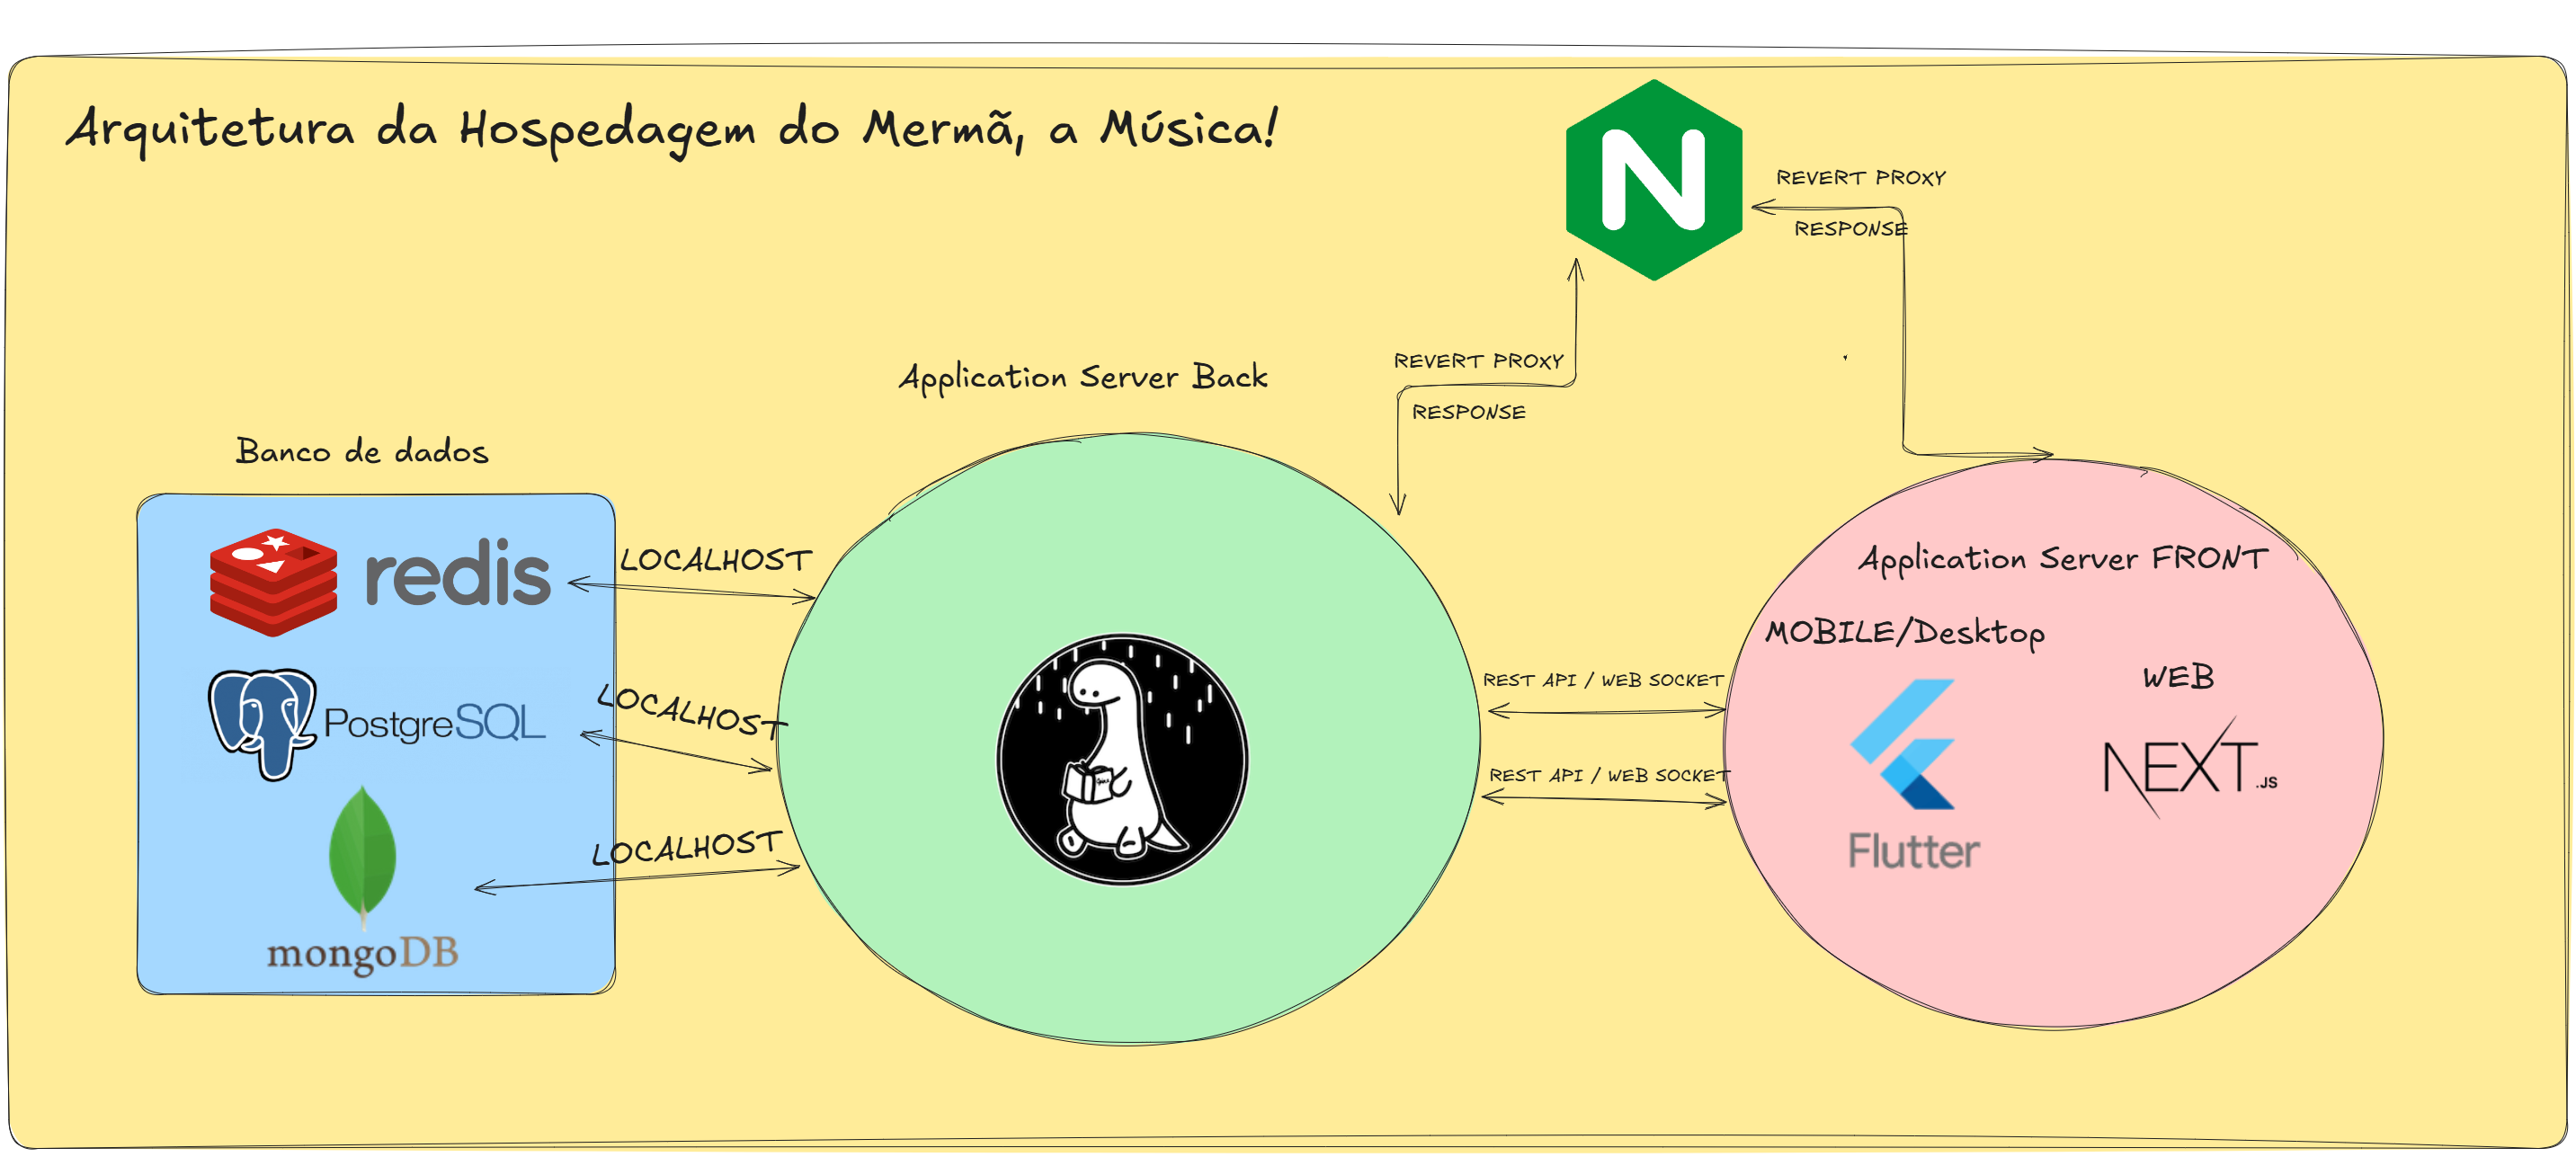
\includegraphics[width=0.8\textwidth]{image/arquitetura_do_projeto.png}
    \caption{Arquitetura do Projeto Mermã, a Música!}
    \label{fig:minha_imagem}
\end{figure}

\subsection{CORE DOMAIN - Sistema de Partidas}
    O Sistema de Partidas é o Core Domain do jogo "Mermã, a Música!", responsável por gerenciar o núcleo da experiência de jogo, desde a criação da partida até a exibição dos resultados finais.  Ele garante a sincronização em tempo real entre os jogadores, oferecendo uma experiência multiplayer fluida e dinâmica.
    \subsubsection{Bounded Context}
    \begin{itemize}
        \item Gerenciamento de Partidas: Responsável por criar, configurar e gerenciar o ciclo de vida das partidas, desde o momento em que são criadas até a finalização e exibição dos resultados.  Isso inclui o controle do estado da partida, gerenciamento de jogadores participantes, e aplicação das regras do modo de jogo selecionado.
        \item Seleção e Reprodução de Músicas: Este contexto lida com a seleção aleatória de músicas a partir das playlists dos jogadores, de acordo com as configurações da partida.  Ele também é responsável por reproduzir os trechos das músicas para os jogadores adivinharem, garantindo a sincronização entre os jogadores.
        \item Registro de Respostas e Pontuação: Responsável por capturar, validar e processar as respostas dos jogadores durante as rodadas.  Ele aplica as regras de acerto (nome da música, artista ou ambos) e calcula a pontuação de cada jogador com base no tempo de resposta e acertos.
        \item Ranking e Progressão: Gerencia o ranking dos jogadores dentro das partidas e no sistema como um todo.  Isso inclui o cálculo do ELO em partidas ranqueadas, atualização do ranking global e progressão dos jogadores nos níveis.
        \item Sincronização em Tempo Real: Este contexto garante que todos os jogadores estejam sincronizados durante a partida, utilizando WebSockets para enviar e receber eventos em tempo real, como atualização do placar, mensagens de chat e status da partida.
    \end{itemize}

\subsubsection{Gerenciamento de Partidas}

O Bounded Context "Gerenciamento de Partidas" é o coração do domínio "Sistema de Partidas", responsável por orquestrar todo o ciclo de vida de uma partida no jogo "Mermã, a Música!". Ele garante que as partidas sejam criadas, configuradas, iniciadas, jogadas e finalizadas de acordo com as regras estabelecidas.
\subsubsection{Responsabilidades}
    \begin{itemize}
        \item \textbf{Criação e Configuração}: Permite aos jogadores criar novas partidas, definindo o modo de jogo (casual, ranqueado, battle royale), as configurações (número de rodadas, tempo de resposta, tipo de acerto, playlists) e os jogadores participantes.
        \item \textbf{Gerenciamento do Ciclo de Vida}: Controla o estado da partida, desde a fase de "aguardando jogadores" até a finalização, passando pelos estados "em andamento", "pausada" e "cancelada".
        \item \textbf{Controle de Jogadores}: Gerencia a entrada e saída de jogadores na partida, garantindo que o número máximo de jogadores não seja excedido e que todos estejam prontos para iniciar.
        \item \textbf{Gerenciamento de Rodadas}: Divide a partida em rodadas, controla o tempo limite para cada rodada e garante a transição suave entre as rodadas.
        \item \textbf{Aplicação de Regras}: Aplica as regras específicas de cada modo de jogo, como o sistema de pontuação, o número de vidas no modo Battle Royale e os critérios de vitória.
        \item \textbf{Finalização e Ranking}: Finaliza a partida quando todas as rodadas forem concluídas ou quando algum critério de finalização for atingido, gera o ranking final da partida e, no caso de partidas ranqueadas, atualiza o ELO dos jogadores.  
    \end{itemize}

\subsubsection{entidades}
    \begin{itemize}
        \item \textbf{Partida}: Representa uma instância do jogo em andamento, armazenando informações sobre o modo de jogo, configurações, estado, jogadores, rodadas, ranking e datas de criação, início e fim.
        \item \textbf{JogadorPartida}:  Representa um jogador dentro de uma partida específica, armazenando sua pontuação, respostas, vidas (no modo Battle Royale), tempo médio de resposta e estado (ativo, eliminado, desconectado).
        \item \textbf{Sala}: Representa o ambiente virtual onde os jogadores se reúnem antes de iniciar uma partida, armazenando informações sobre o nome da sala, dono, jogadores, configurações da partida, tipo de sala (pública ou privada), número máximo de jogadores, código de convite e estado.
    \end{itemize}

\subsubsection{Objetos de Valor}
    \begin{itemize}
        \item \textbf{ConfiguracoesPartida}: Armazena as configurações da partida, como o tipo de acerto (música, artista ou ambos), número de rodadas, tempo limite para resposta, playlists selecionadas e visibilidade da sala.
        \item \textbf{RankingPartida}: Armazena o ranking final da partida, com a lista de jogadores classificados por pontuação, o vencedor, o modo de ranking (normal ou ranqueado) e as variações de ELO (apenas para partidas ranqueadas).
    \end{itemize}

    \begin{figure}[H]
        \centering
        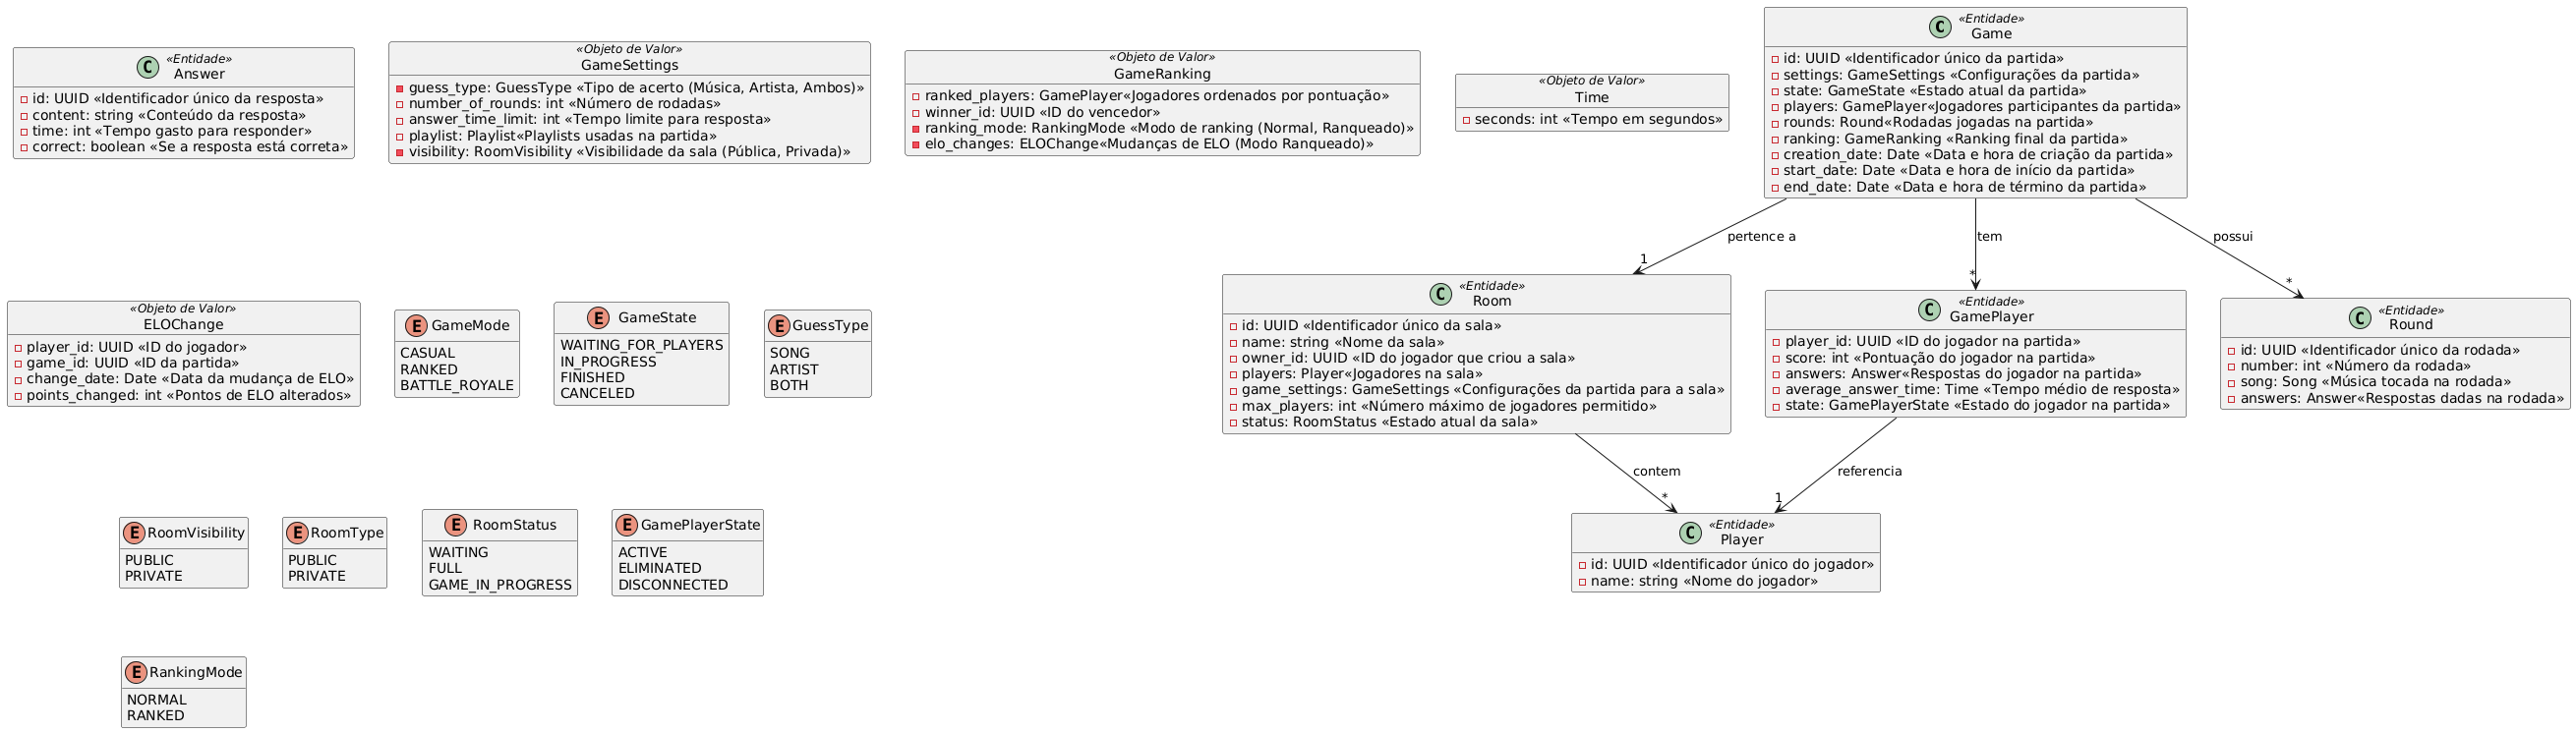
\includegraphics[width=0.8\textwidth]{image/entidades_gerenciamento_partida.png}
        \caption{Entidades do Bounded Context "Gerenciamento de Partidas"}
        \label{fig:minha_imagem}
    \end{figure}

\subsubsection{Relações com outros Bounded Context}
    \begin{itemize}
        \item \textbf{Cliente do contexto "Seleção e Reprodução de Músicas"}: Solicita músicas para serem utilizadas nas rodadas da partida.
        \item \textbf{Fornecedor para os contextos "Registro de Respostas e Pontuação", "Ranking e Progressão" e "Sincronização em Tempo Real"}: Envia informações sobre as respostas dos jogadores, o fim da partida e outros eventos relevantes para esses contextos.
    \end{itemize}

\subsubsection{Caso de Uso 1: Criar uma Partida}
    \textbf{Ator Principal}: Jogador \\
    \textbf{Objetivo}: Criar uma nova sala de espera para iniciar uma partida com outros jogadores, definindo as configurações da partida e a visibilidade da sala. \\
    \textbf{Pre-Requesito}: O jogador deve estar autenticado no sistema. \\
    \textbf{Fluxo Principal}: \\
    \begin{enumerate}
        \item O jogador solicita a criação de uma nova sala.
        \item O sistema solicita ao jogador que defina as configurações da partida: \\
         \subitem \textbf{Modo de Jogo}: 
            \subsubitem Casual: Sem ranking, apenas para diversão. 
            \subsubitem Ranqueado: Partida competitiva que afeta o ranking do jogador. 
            \subsubitem Battle Royale: Partida eliminatória onde o último jogador restante vence.
        \subitem \textbf{Número de Rodadas}: Campo numérico para definir a quantidade de rodadas da partida (valor mínimo: 1, valor máximo: 20).
        \subitem \textbf{Tempo Limite de Resposta}: Seletor de tempo com opções pré-definidas: (5 segundos, 10 segundos, 15 segundos, 20 segundos) ou campo numérico para definir o tempo limite para responder a cada pergunta (valor mínimo: 5 segundos, valor máximo: 30 segundos).
        \subitem \textbf{Tipo de Acerto}: \\
            \subsubitem \textbf{Música}: O jogador precisa acertar apenas o nome da música.
            \subsubitem \textbf{Artista}: O jogador precisa acertar apenas o nome do artista.
            \subsubitem \textbf{Ambos}: O jogador precisa acertar o nome da música e do artista.
        \subitem \textbf{Visibilidade da Sala}: \\
            \subsubitem \textbf{Pública}: Qualquer jogador pode entrar na sala.
            \subsubitem \textbf{Privada}: Apenas jogadores convidados ou com a senha de acesso podem entrar na sala.
        \item O jogador define as configurações desejadas.
        \item Se o jogador escolher "Privada", o sistema solicita que ele defina uma senha de 4 dígitos para a sala.
        \item O jogador define a senha da sala, caso não pula esse passo.
        \item O sistema valida as configurações.
        \item Se as configurações forem válidas, o sistema cria uma nova sala com as configurações definidas, o jogador como dono e a senha caso seja privada.
        \item O sistema adiciona o jogador à sala.
        \item O sistema informa ao jogador que a sala foi criada com sucesso, incluindo o nome da sala e a senha.
    \end{enumerate}

    \textbf{REGRAS DE NEGOCIO}:
    \begin{itemize}
        \item \textbf{Sala Cheia}: Um jogador não pode entrar em uma sala que já atingiu o número máximo de jogadores definido na criação da sala.
        \item \textbf{Partida Iniciada}: Um jogador não pode entrar em uma sala se a partida já tiver sido iniciada.
        \item \textbf{Senha da Sala}
            \subitem A senha deve ter exatamente 4 dígitos sendo todos numericos.
            \subitem Para salas públicas, qualquer jogador pode entrar sem necessidade de senha.
            \subitem Para salas privadas, o jogador precisa fornecer a senha correta para entrar.
            \subitem Se o jogador fornecer uma senha incorreta, o sistema deve exibir uma mensagem de erro e impedir a entrada na sala.
        \item \textbf{Jogador já na Sala}:  Um jogador não pode entrar em uma sala na qual ele já está presente.
        \item \textbf{Estado do Jogador}: 
            \subitem Um jogador não pode entrar em uma sala se estiver banido ou suspenso.
            \subitem Um jogador que foi desconectado de uma partida em andamento pode reentrar na mesma sala, caso a partida ainda esteja acontecendo.
            \subitem O criador da sala é classificado como dono da sala
            \subitem O dono da sala pode definir configurações adicionais, como expulsar jogadores, iniciar a partida e alterar as configurações da sala.
            \subitem O dono da sala sair da sala, a liderança é trasferida para outro jogador presente na sala.
            \subitem O dono da sala pode trasferir a liderança para outro jogador presente na sala.
        \item \textbf{Disponibilidade da Sala}: 
            \subitem Uma sala pode ser removida da lista de salas disponíveis se a partida for iniciada ou se o dono da sala a cancelar.
            \subitem Uma sala privada pode ser removida da lista de salas disponíveis se o dono da sala a fechar ou se tornar inacessível após um determinado tempo de inatividade.
        \item \textbf{Conexão com a Sala}:
            \subitem O sistema deve garantir que o jogador tenha uma conexão estável com a sala.
            \subitem Se o jogador perder a conexão com a sala, ele deve ser removido da lista de jogadores e notificado.
            \subitem O sistema deve tentar reconectar o jogador automaticamente, caso a conexão seja perdida temporariamente.     
    \end{itemize}
\subsubsection{Caso de Uso 2: Entrar em uma Sala}
    \textbf{Ator Principal}: Jogador \\
    \textbf{Objetivo}: Entrar em uma sala de espera existente para participar de uma partida. \\
    \textbf{Pre-Requesito}: O jogador deve estar autenticado no sistema. \\
    \textbf{Fluxo Principal}: \\
    \begin{enumerate}
        \item O jogador solicita a entrada em uma sala, informando o nome ou código da sala.
        \item O sistema verifica se a sala existe.
        \item Se a sala existir, o sistema verifica se ela é pública ou privada.
        \item Se a sala for privada, o sistema solicita a senha ao jogador.
        \item O jogador informa a senha da sala (se solicitada).
        \item O sistema verifica se a senha está correta (se aplicável).
        \item O sistema verifica se a sala ainda não está cheia e se a partida ainda não foi iniciada.
        \item Se a sala estiver disponível, o sistema adiciona o jogador à sala.
        \item O sistema informa ao jogador que ele entrou na sala com sucesso.
        \item O sistema notifica os demais jogadores na sala sobre a entrada do novo jogador.
    \end{enumerate}

    \textbf{REGRAS DE NEGOCIO}:
    \begin{itemize}
        \item \textbf{Sala Cheia}: Um jogador não pode entrar em uma sala que já atingiu o número máximo de jogadores.
        \item \textbf{Partida Iniciada}: Um jogador não pode entrar em uma sala se a partida já tiver sido iniciada.
        \item \textbf{Senha da Sala}:
            \subitem Salas públicas podem ser acessadas por qualquer jogador sem senha.
            \subitem Salas privadas exigem a senha correta para acesso.
            \subitem Se a senha estiver incorreta, o sistema informa o erro ao jogador e impede a entrada na sala.
        \item \textbf{Jogador já na Sala}: Um jogador não pode entrar em uma sala na qual ele já está presente.
        \item \textbf{Estado do Jogador}:  Um jogador banido ou suspenso não pode entrar em uma sala. 
    \end{itemize}
\subsubsection{Caso de Uso 3: Iniciar Partida}
    \textbf{Ator Principal}: Lider da Sala \\
    \textbf{Objetivo}: Iniciar a partida na sala de espera, após a configuração da partida e a entrada dos jogadores. \\
    \textbf{Pre-Requesito}: O lider da sala tem está em uma sala e todos os jogadores tem que está com estado de "pronto" \\
    \textbf{Fluxo Principal}: \\
    \begin{enumerate}
        \item O dono da sala clica no botão "Iniciar Partida".
        \item O sistema verifica se há pelo menos dois jogadores na sala.
        \item O sistema verifica se todos os participantes então em estado de "pronto"
        \item Se houver jogadores suficientes, o sistema altera o estado da sala para "Partida em Andamento".
        \item O sistema cria uma nova instância de Partida com as configurações definidas na sala.
        \item O sistema associa os jogadores da sala à instância da Partida.
        \item O sistema obtém as playlists dos jogadores participantes.
        \item O sistema inicia a primeira rodada da partida.
        \item O sistema notifica todos os jogadores da sala que a partida foi iniciada.
        \item O sistema redireciona todos os jogadores para a tela da partida.
    \end{enumerate}

    \textbf{REGRAS DE NEGOCIO}:
    \begin{itemize}
        \item \textbf{Número Mínimo de Jogadores}: Uma partida só pode ser iniciada se houver pelo menos dois jogadores na sala.
        \item \textbf{Todos os jogadores devem está prontos}: A partida só inicia quando todos os jogadores estão em estado de "pronto".
        \item \textbf{Lider da Sala Inicia}: Apenas o Lider da Sala pode iniciar a partida.
        \item \textbf{Estado da Sala}: A sala deve estar no estado "Aguardando Jogadores" para que a partida possa ser iniciada.
    \end{itemize}
\subsubsection{Caso de Uso 4: Responder a uma Pergunta}
    \textbf{Ator Principal}: Jogador  \\
    \textbf{Objetivo}: Responder a uma pergunta sobre a música que está sendo tocada na rodada atual da partida, com a possibilidade de múltiplas tentativas até o tempo limite. \\
    \textbf{Pre-Requesito}: A partida tem que ser válida e está em andamento \\
    \textbf{Fluxo Principal}: \\
    \begin{enumerate}
        \item O sistema apresenta uma pergunta ao jogador sobre a música que está sendo tocada na rodada atual.
        \item O jogador analisa a pergunta e as opções de resposta.
        \item O jogador seleciona a opção de resposta que acredita ser a correta.
        \item O sistema registra a resposta do jogador e o tempo em que ela foi dada.
        \item O jogador pode continuar respondendo à mesma pergunta, alterando sua resposta quantas vezes desejar, até o tempo limite.
        \item Quando o tempo limite da rodada expirar, o sistema considera a última resposta dada pelo jogador como a resposta final.
        \item O sistema verifica se a resposta final do jogador está correta.
        \item Se a resposta final estiver correta, o sistema calcula a pontuação do jogador com base no tempo da última resposta.
        \item O sistema atualiza a pontuação do jogador na partida.
        \item O sistema notifica o jogador sobre o resultado da sua resposta final (correta ou incorreta) e a pontuação obtida.
        \item O sistema verifica se a rodada terminou (todos os jogadores responderam ou o tempo limite da rodada expirou).
        \item Se a rodada terminou, o sistema inicia a próxima rodada ou finaliza a partida, caso seja a última rodada.
    \end{enumerate}
    \textbf{REGRAS DE NEGOCIO}:
    \begin{itemize}
        \item \textbf{Tempo Limite}:O jogador tem um tempo limite para responder a cada pergunta, definido nas configurações da partida.
        \item \textbf{Múltiplas Tentativas}:O jogador pode responder à mesma pergunta várias vezes dentro do tempo limite.
        \item \textbf{Última Resposta}: O sistema considera apenas a última resposta dada pelo jogador como a resposta final.
        \item \textbf{Pontuação}: A pontuação do jogador é calculada com base no tempo da última resposta e no tipo de acerto (música, artista ou ambos), conforme definido nas configurações da partida.
        \item \textbf{Tipo de Pergunta}: O tipo de pergunta (música, artista ou ambos) varia de acordo com as configurações da partida.
        \item \textbf{Registro de tempo de resposta}: O sistema deve registrar todas as respostas do jogador e seus respectivos tempos, mas apenas a última resposta é considerada para o cálculo da pontuação.
    \end{itemize}
\subsubsection{Caso de Uso 5: Finalizar Rodada}
    \textbf{Ator Principal}: Sistema  \\
    \textbf{Objetivo}: inalizar uma rodada da partida, calcular a pontuação dos jogadores e determinar o próximo passo do jogo (próxima rodada ou finalização da partida). \\
    \textbf{Pre-Requesito}: A partida tem que ser válida e está em andamento \\
    \textbf{Fluxo Principal}: \\
    \begin{enumerate}
        \item O sistema aguarda até que todos os jogadores tenham respondido à pergunta da rodada ou o tempo limite da rodada expire.
        \item O sistema verifica as respostas de cada jogador e calcula a pontuação individual de acordo com as regras de pontuação definidas nas configurações da partida.
        \item O jogador seleciona a opção de resposta que acredita ser a correta.
        \item O sistema atualiza a pontuação total de cada jogador na partida.
        \item O sistema exibe o resultado da rodada para todos os jogadores, incluindo a resposta correta, a pontuação de cada jogador e o ranking da rodada.
        \item O sistema verifica se a rodada finalizada era a última rodada da partida.
        \item Se houver mais rodadas, o sistema inicia a próxima rodada.
        \item Se a rodada finalizada era a última, o sistema finaliza a partida.
    \end{enumerate}
    
    \textbf{REGRAS DE NEGOCIO}:
    \begin{itemize}
        \item \textbf{Término da Rodada}: Uma rodada termina quando todos os jogadores responderam à pergunta ou o tempo limite da rodada expirou.
        \item \textbf{Cálculo da Pontuação}:A pontuação de cada jogador é calculada com base em sua resposta e no tempo gasto para responder, conforme definido nas configurações da partida.
        \item \textbf{Ranking da Rodada}:O sistema classifica os jogadores de acordo com sua pontuação na rodada.
        \item \textbf{Pontuação}: A pontuação do jogador é calculada com base no tempo da última resposta e no tipo de acerto (música, artista ou ambos), conforme definido nas configurações da partida.
        \item \textbf{Progressão da Partida}: O sistema controla a progressão da partida, verificando se há mais rodadas a serem jogadas ou se a partida deve ser finalizada.
    \end{itemize}
\subsubsection{Caso de Uso 6: Finalizar Partida}
    \textbf{Ator Principal}: Sistema \\
    \textbf{Objetivo}: Finalizar a partida, calcular o ranking final, atualizar o ELO dos jogadores (se aplicável) e realizar outras ações necessárias ao término da partida. \\
    \textbf{Pre-Requesito}: A partida tem que ser válida e está em andamento \\
    \textbf{Fluxo Principal}: \\
    \begin{enumerate}
        \item O sistema verifica se a última rodada da partida foi finalizada.
        \item Se a última rodada foi finalizada, o sistema calcula a pontuação final de cada jogador.
        \item O sistema gera o ranking final da partida, classificando os jogadores por pontuação.
        \item Se a partida for ranqueada, o sistema atualiza o ELO dos jogadores com base em seus resultados.
        \item O sistema armazena os resultados da partida, incluindo o ranking final e as pontuações individuais.
        \item O sistema exibe a tela de resultados da partida para todos os jogadores, mostrando o ranking final, a pontuação de cada jogador e outras estatísticas relevantes.
        \item O sistema encerra a instância da \textbf{Partida}.
        \item O sistema libera os jogadores da sala.
        \item O sistema disponibiliza opções para os jogadores, como:
            \subitem Iniciar uma nova partida fazendo os jogadores voltarem direto para a SALA.
            \subitem Voltar para a tela inicial, fazendo os jogadores voltarem para a seleção de salas ou home.
            \subitem Visualizar o perfil dos jogadores.
            \subitem Compartilhar os resultados nas redes sociais.
    \end{enumerate}
    
    \textbf{REGRAS DE NEGOCIO}:
    \begin{itemize}
        \item \textbf{Finalização da Partida}:A partida é finalizada quando a última rodada é concluída.
        \item \textbf{Cálculo do Ranking}:O ranking final é calculado com base na pontuação total de cada jogador na partida.
        \item \textbf{Atualização do ELO}:Em partidas ranqueadas, o ELO dos jogadores é atualizado de acordo com as regras de cálculo do ELO.
        \item \textbf{Armazenamento dos Resultados}: Os resultados da partida são armazenados para fins de histórico e estatísticas.
    \end{itemize}

\subsubsection{MAPA DE CONTEXTO}
    \begin{figure}[H]
        \centering
        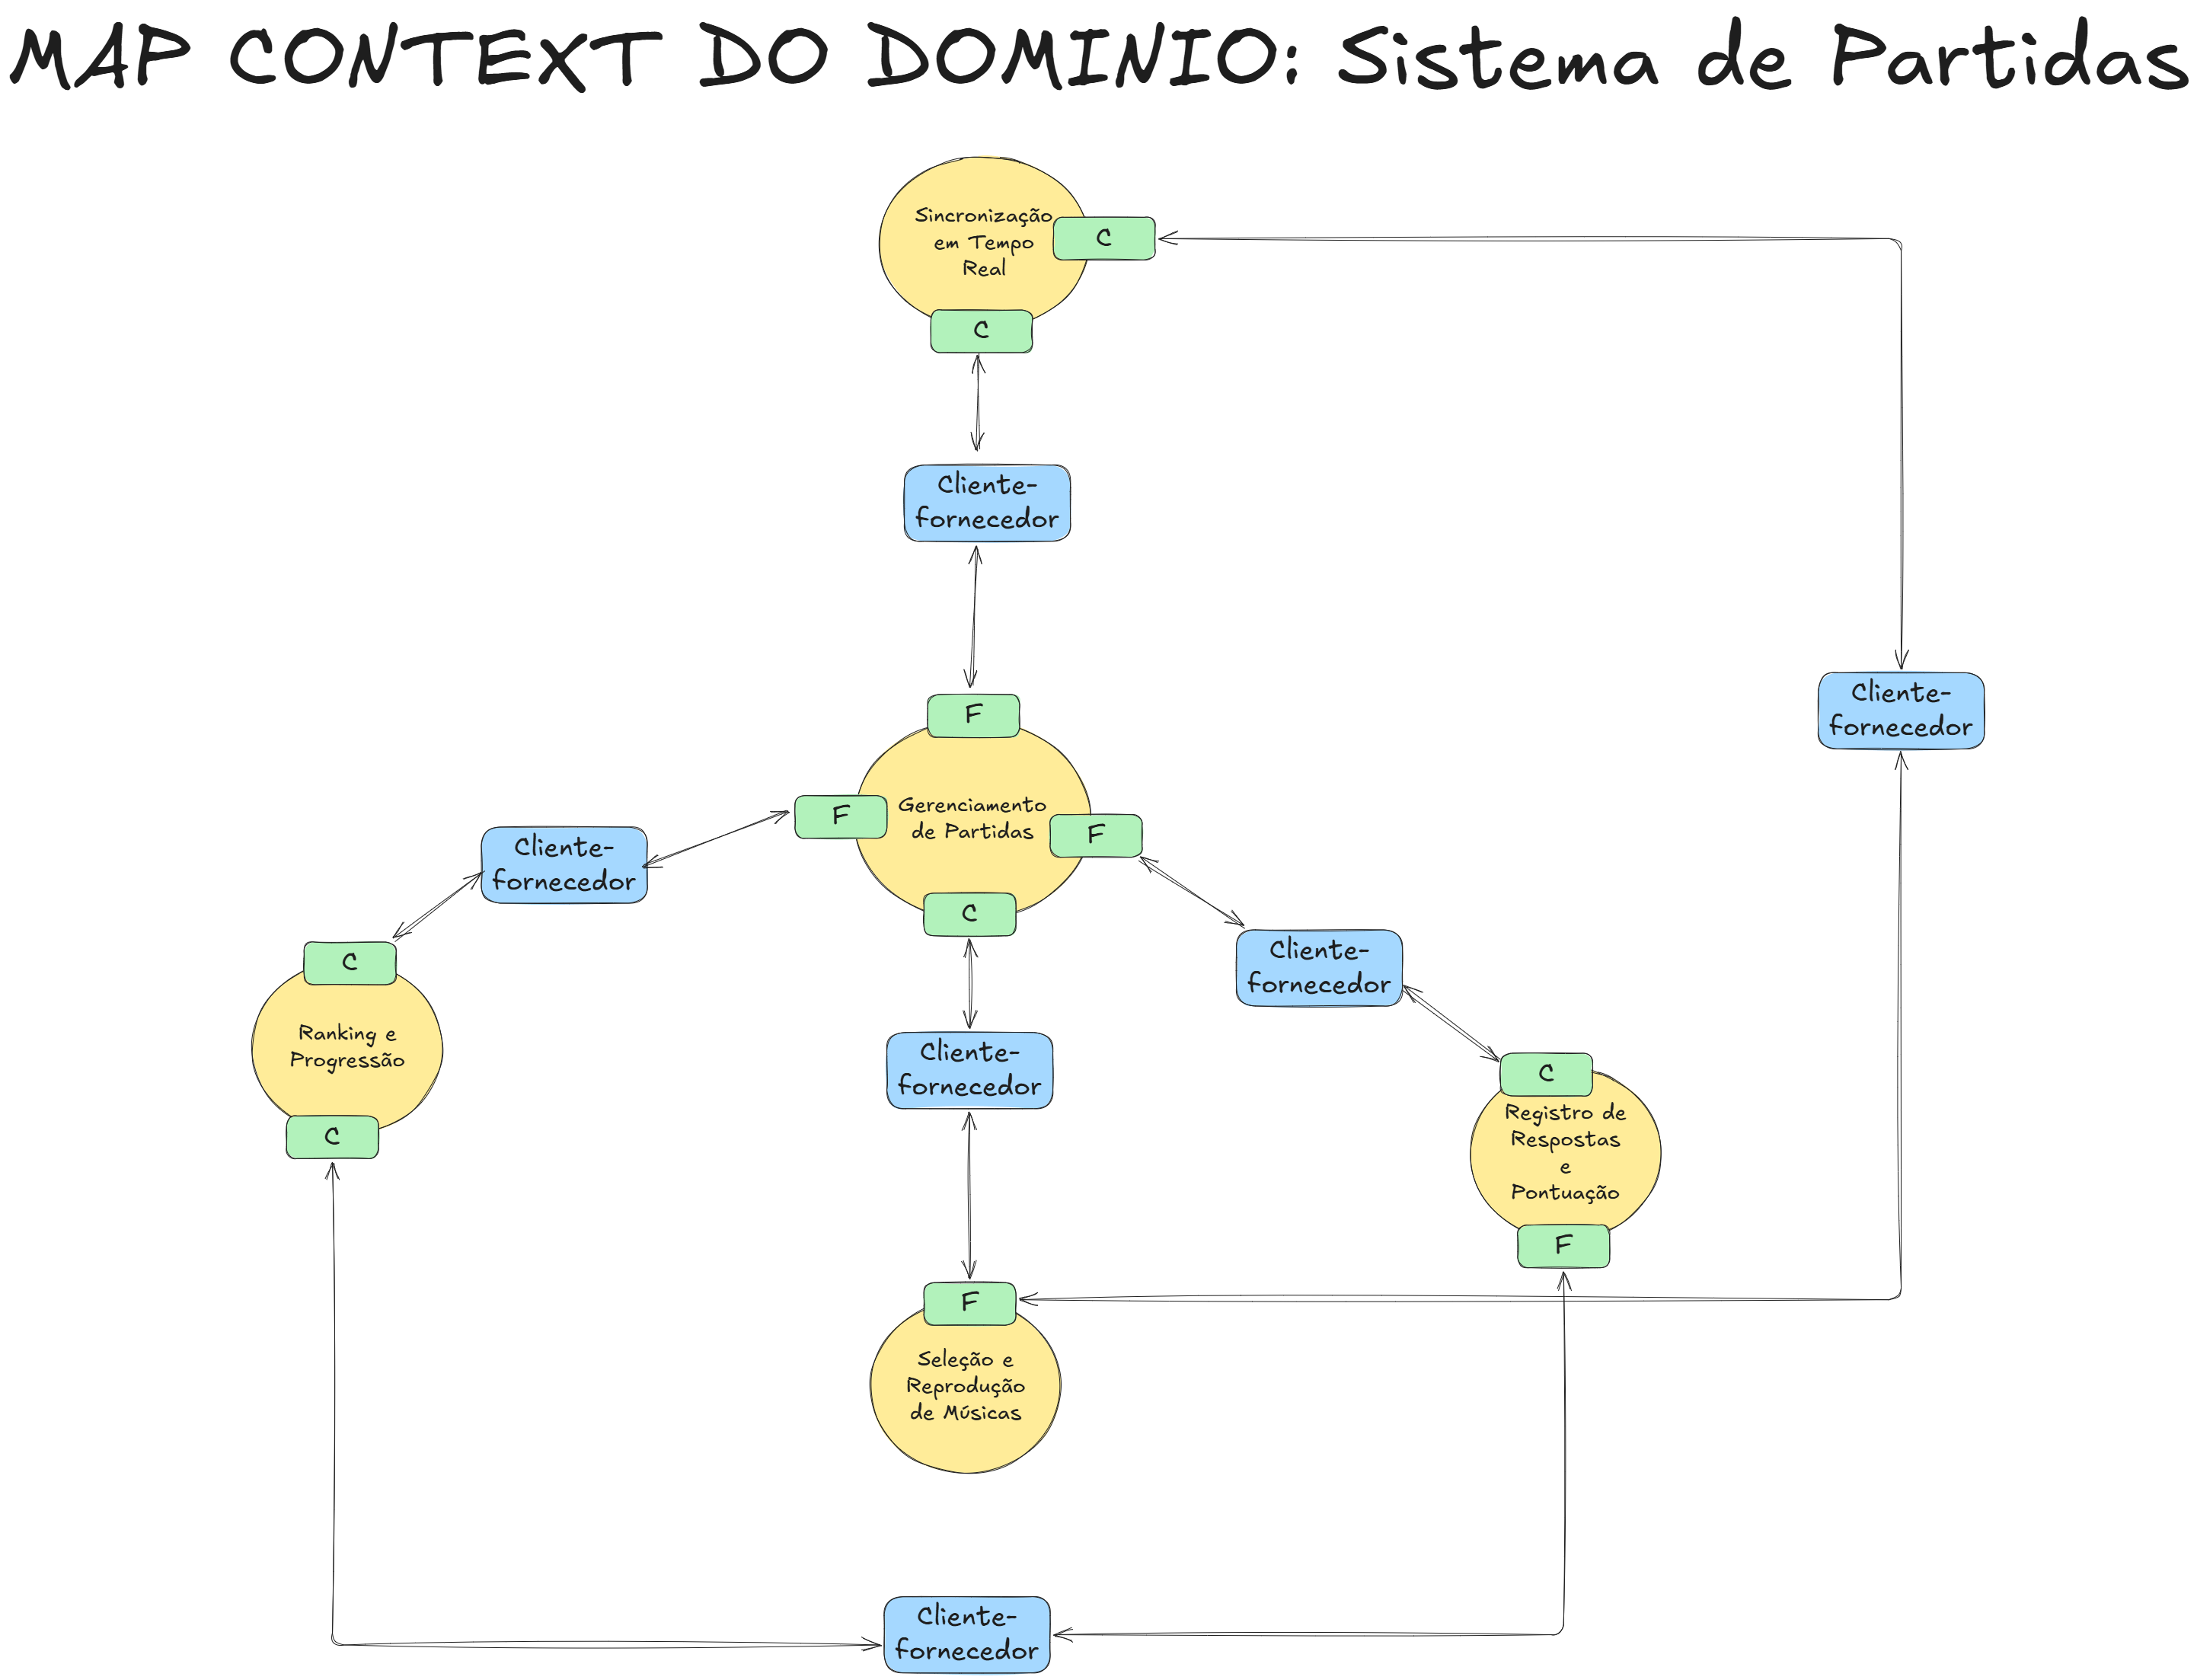
\includegraphics[width=0.8\textwidth]{image/mapa_contexto_sistema_partida.png}
        \caption{Mapa de Contexto do Sistema de Partidas; \\ Cliente - Servidor:  O contexto "Clinte" requesita infomações do contexto "Fornecedor" para realizar suas tarefas. \\ "C" -> Cliente || "F" -> Fornecedor}
        \label{fig:minha_imagem}
    \end{figure}

    

\end{titlepage}


